\section{Introduction}

\paragraph{Problem} I use multiple filaments for my \Printername, often months go by between uses. Spcific types of filament, such as PLA, PETG and nylon degrade as the filament absorbs moisture. To remove the moisture I use a Sunlu filament dryer along with my Ender 3. However, the filament heater positioned beside the printer requires routing filament from table height up and back down to the extruder inlet. The stock filament holder on the Ender 3 does not
accommodate an elevated feed path, causing the filament to bind at the entry point or collide with larger prints.
My current setup can be see in Fig.\ref{fig:CurrentSetup}.



\begin{figure}[tbh!]
	\centering
	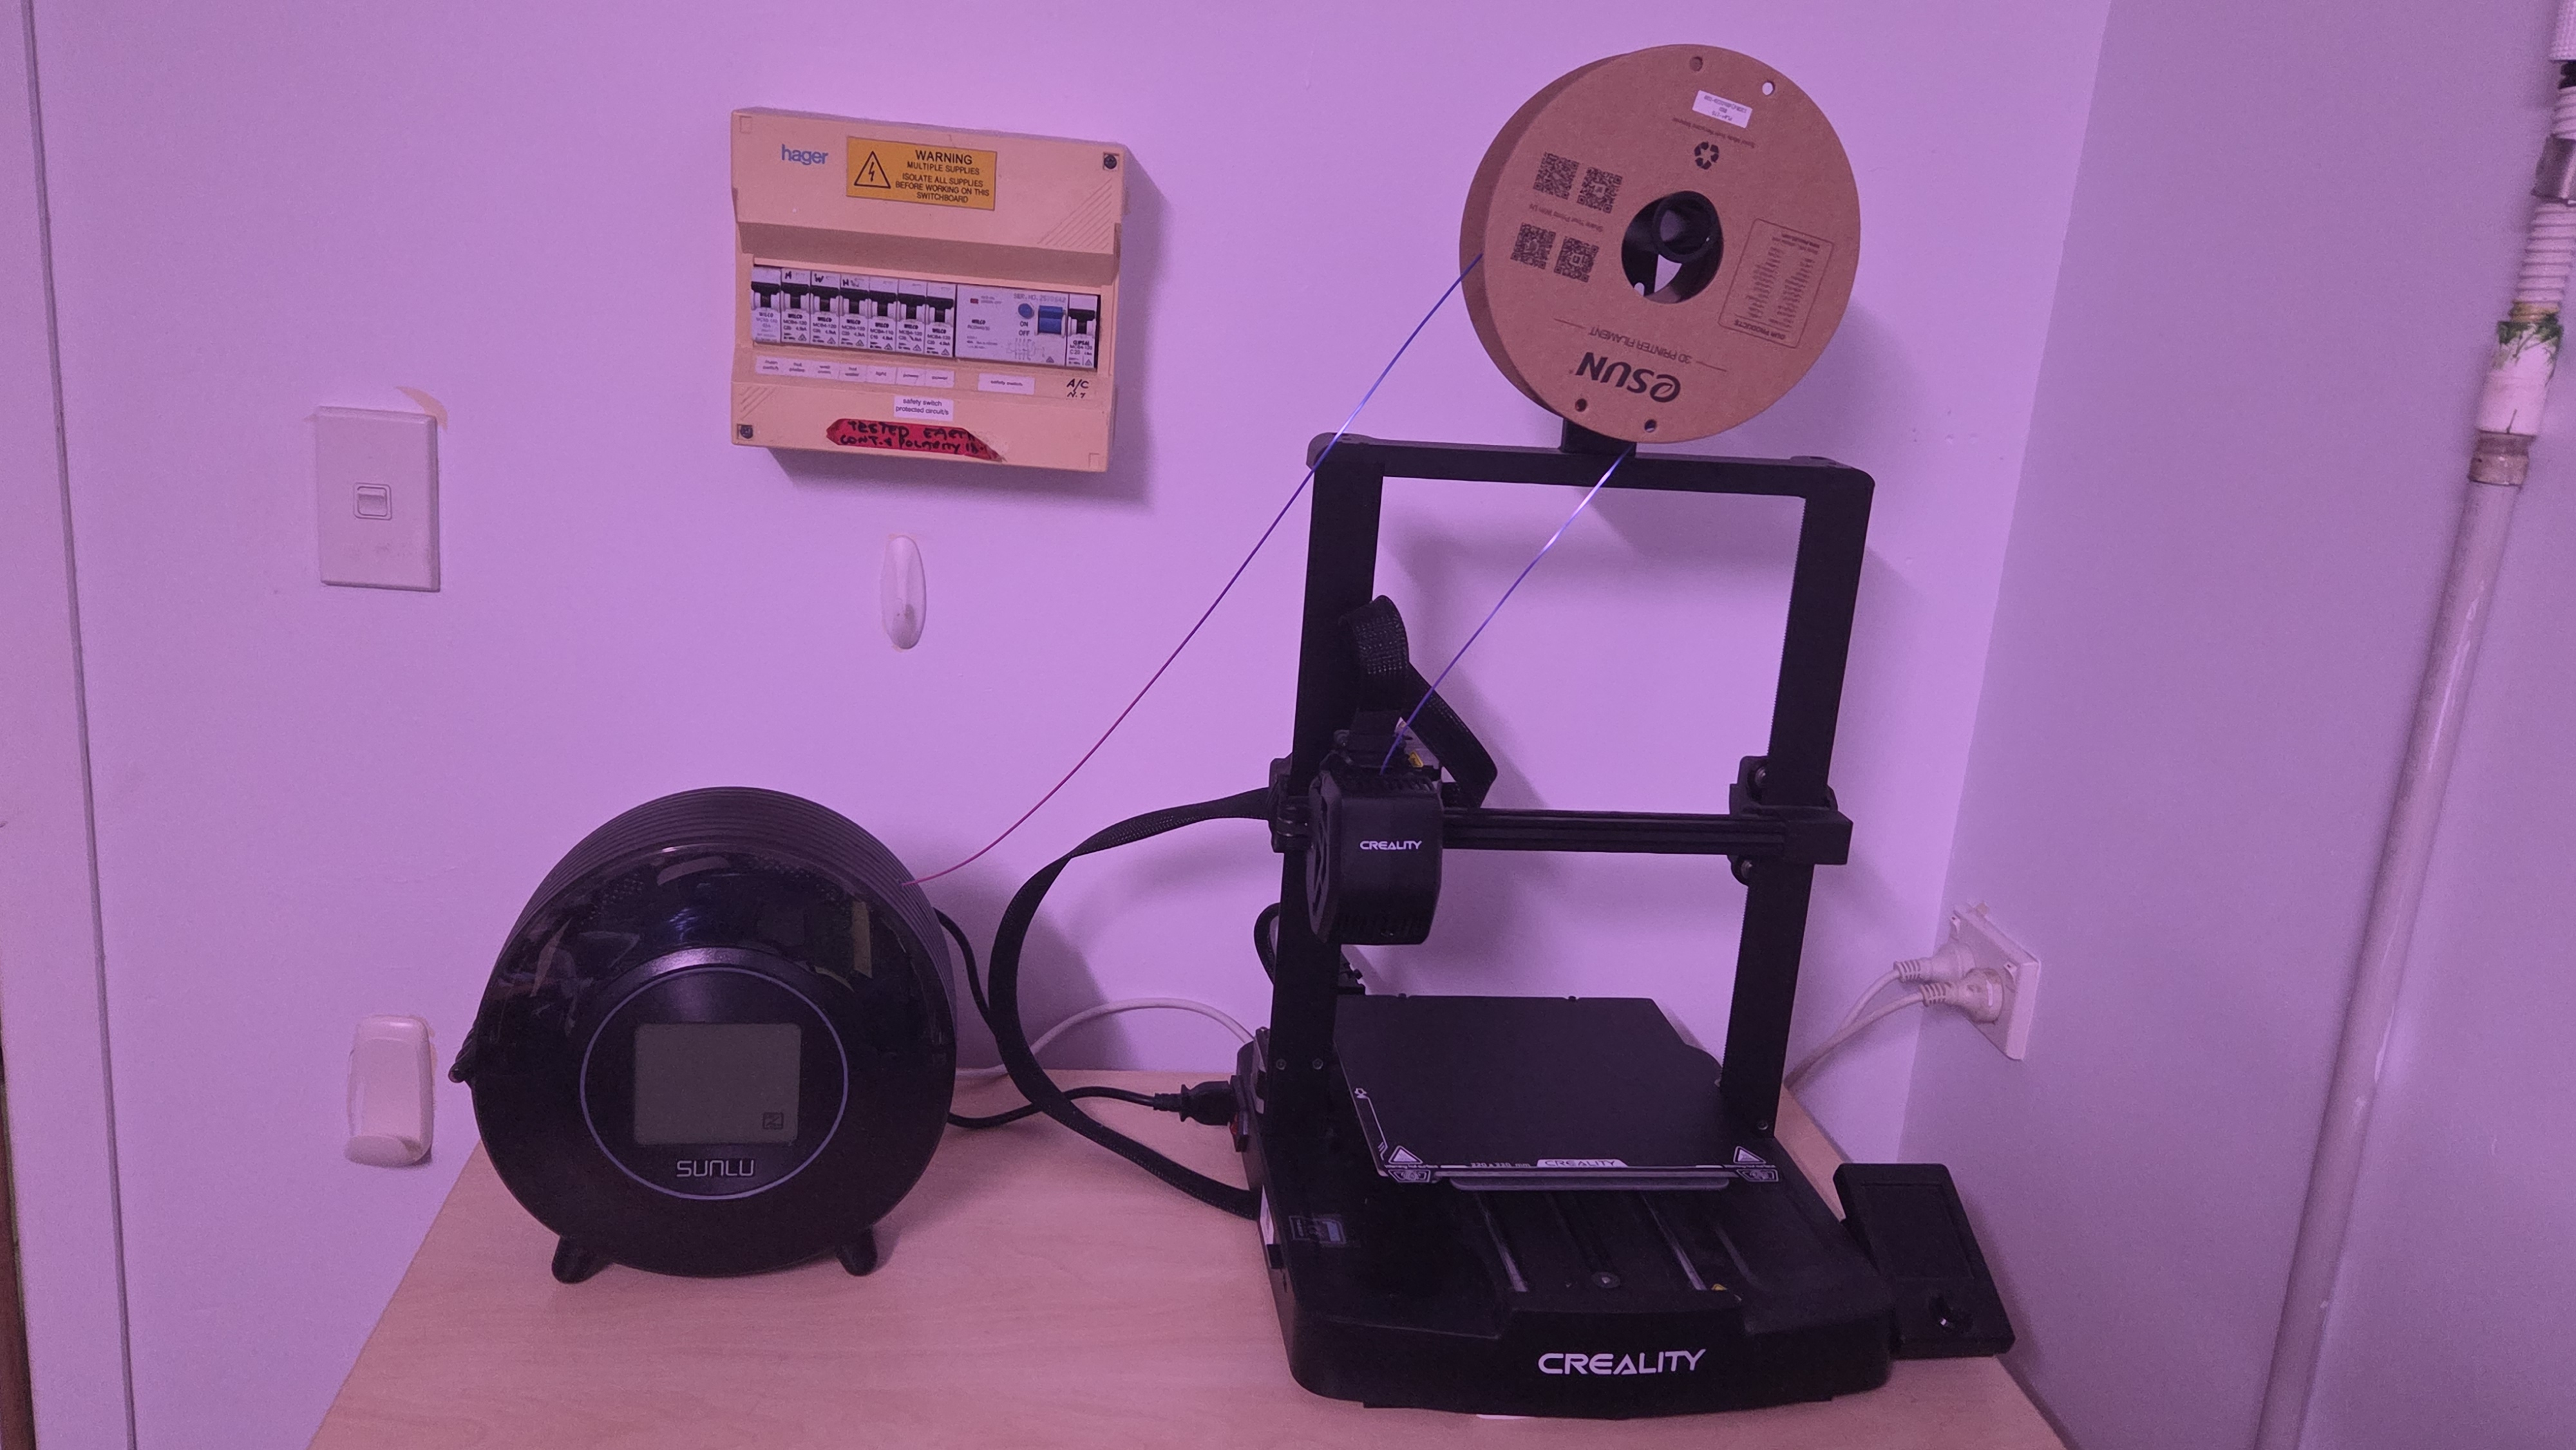
\includegraphics[width={\dimexpr\textwidth - 6pt - 1pt\relax}]{./Images/3DPrintSetup.jpg}
	\caption{My Current \Printername\;setup}\label{fig:CurrentSetup}
\end{figure}




This report documents the design, manufacture, and testing of a 3D
printed filament guide attachment that mounts in place of the stock
holder and provides a smooth, low-friction feed path for the elevated
filament routing configuration.

